\documentclass[tikz,border=2pt]{standalone}
\usepackage{amsmath,amssymb}
\usepackage{tikz}
\usetikzlibrary{arrows.meta}

\begin{document}
% Three stationary points (grad f = 0) seen through their level sets: closed loops around a
% peak (Hessian negative definite: local max), around a pit (positive definite: local min),
% crossing curves at a saddle (indefinite).
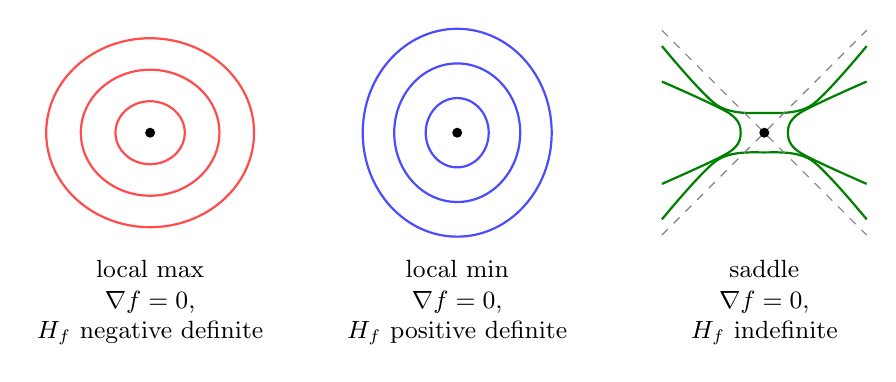
\begin{tikzpicture}[every node/.style={font=\small}]
	\begin{scope}
		\foreach \r in {0.4,0.8,1.2} {\draw[red!70, thick] (0,0) ellipse ({\r*1.1} and {\r});}
		\fill (0,0) circle (1.8pt);
		\node[anchor=north, align=center] at (0,-1.5) {local max\\ $\nabla f=0$,\\ $H_f$ negative definite};
	\end{scope}
	\begin{scope}[xshift=3.9cm]
		\foreach \r in {0.4,0.8,1.2} {\draw[blue!70, thick] (0,0) ellipse ({\r} and {\r*1.1});}
		\fill (0,0) circle (1.8pt);
		\node[anchor=north, align=center] at (0,-1.5) {local min\\ $\nabla f=0$,\\ $H_f$ positive definite};
	\end{scope}
	\begin{scope}[xshift=7.8cm]
		\draw[green!50!black, thick] plot[smooth] coordinates {(-1.3,1.1) (-0.6,0.35) (0,0.25) (0.6,0.35) (1.3,1.1)};
		\draw[green!50!black, thick] plot[smooth] coordinates {(-1.3,-1.1) (-0.6,-0.35) (0,-0.25) (0.6,-0.35) (1.3,-1.1)};
		\draw[green!50!black, thick] plot[smooth] coordinates {(-1.3,0.65) (-0.45,0.25) (-0.3,0) (-0.45,-0.25) (-1.3,-0.65)};
		\draw[green!50!black, thick] plot[smooth] coordinates {(1.3,0.65) (0.45,0.25) (0.3,0) (0.45,-0.25) (1.3,-0.65)};
		\draw[gray, dashed] (-1.3,-1.3) -- (1.3,1.3);
		\draw[gray, dashed] (-1.3,1.3) -- (1.3,-1.3);
		\fill (0,0) circle (1.8pt);
		\node[anchor=north, align=center] at (0,-1.5) {saddle\\ $\nabla f=0$,\\ $H_f$ indefinite};
	\end{scope}
\end{tikzpicture}
\end{document}
